\section{Four Roles, Three Planes, One Research Runtime}
\label{sec:rolesplanes}\label{sec:architecture}\label{sec:roles}

\begin{designbox}
Separate authority two ways at once. Three planes physically divide decision,
execution, and evidence, so judgment and record-keeping can never be confused. Four
persistent roles carry every scientific and scheduling decision across a narrow
typed interface --- a Python dataclass with named fields --- so no role can quietly
reach past its contract.
\end{designbox}

Argus is one research runtime organized as three cooperating planes and driven by
four persistent roles. The \textbf{control plane} holds the roles and scheduler that
decide \emph{what to run and whether it is done}; the \textbf{execution plane} runs
\emph{one mission at a time} against real tools, providers, and budgets; and the
\textbf{evidence plane} records the run on an append-only tape and never decides it.
Figure~\ref{fig:planes} shows the planes and their interfaces, and
Figure~\ref{fig:architecture} is the accepted schematic with the four roles inside
the persistent runtime. Table~\ref{tab:planes} assigns each plane its authority.

\begin{figure}[ht]
\centering
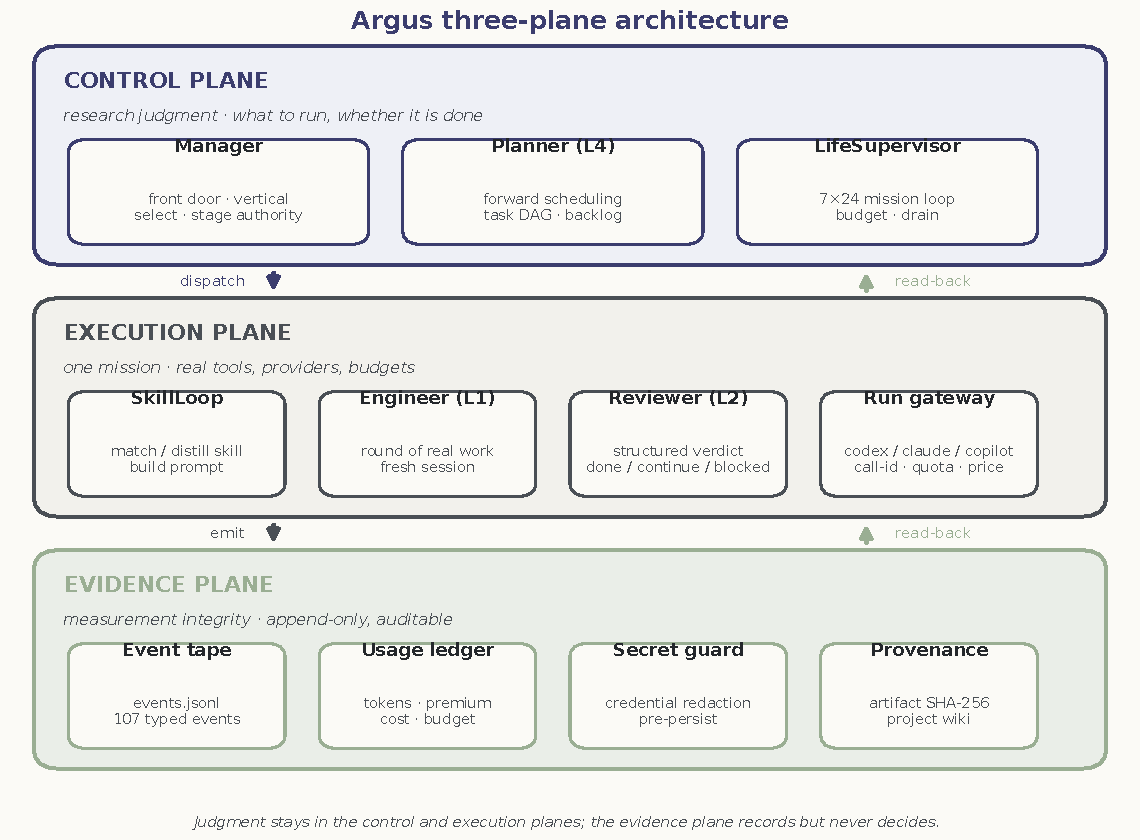
\includegraphics[width=\textwidth]{figures/system_planes.pdf}
\caption{The three-plane architecture. Control-plane roles dispatch work into the
execution plane, which emits typed events into the evidence plane; the evidence
plane is read back by both other planes but holds no decision authority. Drawn
deterministically from the module map (Appendix~\ref{app:evidencemap}).}
\label{fig:planes}
\end{figure}

\begin{table}[h]
\centering
\small
\begin{tabularx}{\linewidth}{@{}p{1.9cm} p{4.6cm} X@{}}
\toprule
\textbf{Plane} & \textbf{Primary components} & \textbf{Authority} \\
\midrule
control &
Manager, Planner, \code{LifeSupervisor}, daemon (\code{manager/}, \code{planner/}, \code{life/}, \code{daemon/}) &
decides what to run and whether a project is done \\
execution &
\code{SkillLoop}, Engineer, Reviewer, provider gateway, verticals (\code{loop.py}, \code{engineer/}, \code{reviewer/}, \code{core/run\_gateway.py}) &
runs one mission; the Reviewer holds mission-level scientific authority \\
evidence &
event tape, usage ledger, secret guard, provenance, wiki (\code{core/}, \code{skills/provenance.py}, \code{wiki/}) &
records and checks; holds no decision authority \\
\bottomrule
\end{tabularx}
\caption{The three planes and their authority. Control and execution decide;
evidence records. Full module map: \srcpath{docs/ARCHITECTURE.md}.}
\label{tab:planes}
\end{table}

The end-to-end control path is a single spine: \code{CLI} $\rightarrow$
\code{Manager.divide} $\rightarrow$ runtime wiring $\rightarrow$ \code{LifeSupervisor}
$\rightarrow$ \code{SkillLoop} $\rightarrow$ \code{SupervisedEngineer}
$\leftrightarrow$ Reviewer-until-done, resting on the core services, the single
anti-stall mechanism, the pluggable verticals, and the provider backend. Every
provider call, regardless of role, is issued through one application-level gateway
(\code{core/run\_gateway.py}) that assigns a \code{call\_id} and stamps timing ---
the single interception point that makes tracing, budgeting, and the per-call audit
of Section~\ref{sec:evidence} possible. The concrete backends (Codex, Claude Code,
Copilot CLI) sit behind an adapter; a deterministic in-memory backend drives tests.

\begin{figure}[ht]
\centering
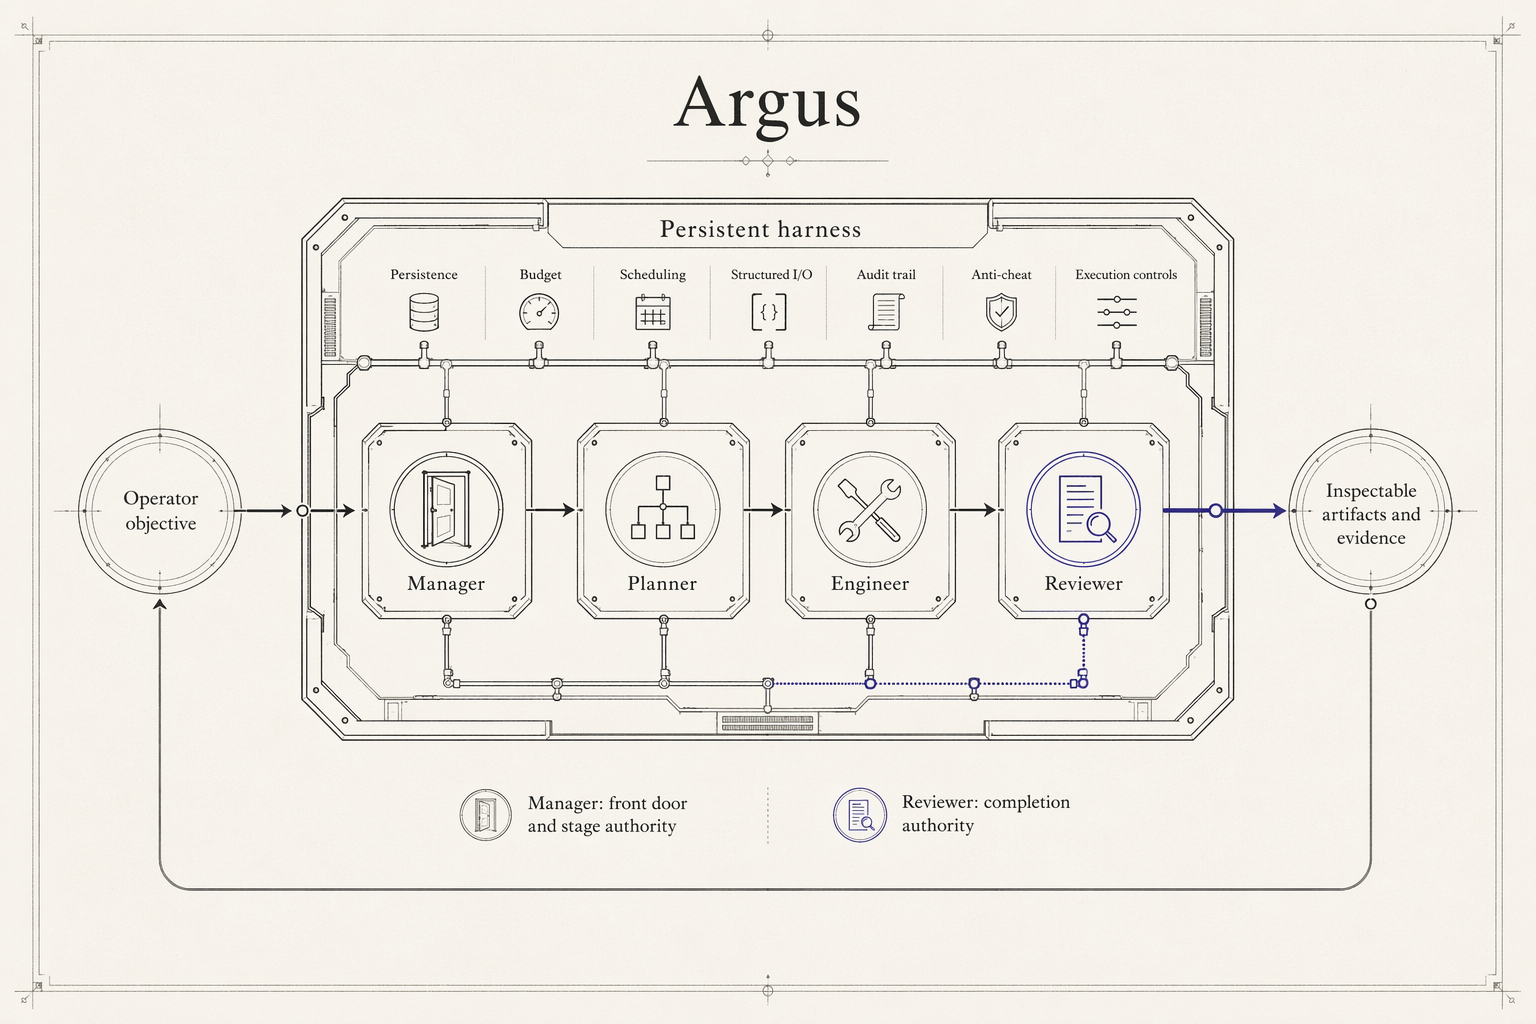
\includegraphics[width=0.6\textwidth]{figures/argus_architecture.png}
\caption{System schematic (not a measured performance plot): an operator objective
enters the persistent runtime; the Manager, Planner, Engineer, and Reviewer sit
inside it as the four roles that carry every research judgment; and inspectable
artifacts and evidence exit back to the operator.}
\label{fig:architecture}
\end{figure}

The four roles below each emit a typed decision interface, so authority is explicit
and verdicts are machine-checkable. Three form a numbered execution spine (Planner
L4, Engineer L1, Reviewer L2); the Manager spans the whole pipeline and sits outside
the numbering. (A fifth role, the Curator, runs only in team/subagent mode and is
out of scope here.)

\subsection{Manager --- front door and stage authority}

The Manager converts operator free text into a committed campaign in a single
grounded model call that emits six structured axes at once --- \code{CONFIG} (a
knob change), \code{CONTROL} (whether to dispatch), \code{ROUTE} (self-reply
vs.\ team task and vertical), \code{LIFETIME} (bounded vs.\ standing),
\code{FAST\_REPLY} (an optional one-line reply), and \code{NAME} (a title). A
\code{CONTROL: NO\_DISPATCH}
decision is authoritative: the bridge forces a read-only self-reply and, if that
fails, fails closed rather than enqueuing work. A task division yields a
\code{Division}; stage progression is a \code{StageTransition}
(Table~\ref{tab:manager}). The Manager is the sole writer of \code{current\_stage};
the transition's \code{action} and \code{source} fields make the decision and
its justification auditable, including fail-safe holds when a downstream role is
unavailable. The other roles may advise a stage change but never write it.

\begin{table}[h]
\centering
\small
\begin{tabularx}{\linewidth}{@{}p{2.4cm} p{2.6cm} X@{}}
\toprule
\textbf{Field} & \textbf{Type / values} & \textbf{Meaning} \\
\midrule
\multicolumn{3}{@{}l}{\textit{Division} \; \code{manager/\_core.py}} \\
\code{task}     & str  & the committed objective text \\
\code{vertical} & str  & the one selected task shape (never re-classified) \\
\code{stages}   & list & the vertical's ordered stage template \\
\addlinespace
\multicolumn{3}{@{}l}{\textit{StageTransition} \; \code{manager/\_core.py}} \\
\code{action}   & advance $\vert$ hold $\vert$ rollback $\vert$ complete & the move applied to \code{current\_stage} \\
\code{source}   & manager\_llm $\vert$ *\_hold & a model decision, or a fail-safe hold \\
\bottomrule
\end{tabularx}
\caption{Manager decision interface. Only the Manager mutates
\code{current\_stage}; a \code{hold} writes nothing.}
\label{tab:manager}
\end{table}

\subsection{Planner (L4) --- forward scheduling}

When the backlog empties in continuous mode, the Planner proposes the next batch of
work as a set of \code{TaskSpec}s and returns a \code{PlannerVerdict}
(Table~\ref{tab:planner}). Tasks form an optional DAG --- each \code{TaskSpec} has a
local \code{key} and a \code{deps} list the scheduler maps to real backlog ids ---
and each carries a structured \code{scope} threaded to the Reviewer as a backlog
tag, so completion authority never re-parses prose to learn a task's scope. The
verdict also has a first-class \code{waiting} outcome (with a durable
\code{WaitingContract}) for a project correctly blocked on a live external job with
no genuinely new high-impact work to queue. The Planner is the sole plan author; the
Reviewer may only report that new evidence has overtaken the current plan.

\begin{table}[h]
\centering
\small
\begin{tabularx}{\linewidth}{@{}p{2.6cm} p{2.5cm} X@{}}
\toprule
\textbf{Field} & \textbf{Type} & \textbf{Meaning} \\
\midrule
\multicolumn{3}{@{}l}{\textit{TaskSpec} \; \code{planner/planner.py}} \\
\code{title, objective} & str & human title + full actionable description \\
\code{impact\_score}    & int 0--5 & parser accepts only high-value work \\
\code{scope}            & bounded $\vert$ final\_submission & threaded to the Reviewer as a tag \\
\code{key, deps}        & str, list & DAG node id and its dependencies \\
\addlinespace
\multicolumn{3}{@{}l}{\textit{PlannerVerdict} \; \code{planner/planner.py}} \\
\code{project\_done}    & bool & project-level completion proposal \\
\code{new\_tasks}       & list & the next batch \\
\code{waiting}          & bool & intentional idle on a live external blocker \\
\code{restart\_daemon}  & bool & request a controlled daemon restart \\
\code{checklist\_ops}   & list & per-stage checklist edits (Planner owns it) \\
\bottomrule
\end{tabularx}
\caption{Planner decision interface (abridged). Scope is structured, never inferred
from the objective text.}
\label{tab:planner}
\end{table}

\subsection{Engineer (L1) --- one round of real work}

The Engineer executes a single round against real tools and hardware. Its interface
to a provider is the per-call \code{RunnerOptions} contract, and it receives back a
\code{RunnerResult} (Table~\ref{tab:engineer}). Two properties matter for integrity.
First, provider-side spend fences (\code{max\_budget\_usd}, \code{max\_ai\_credits})
are populated from an atomic budget \emph{reservation}, not from role configuration,
so a role cannot raise its own ceiling (Section~\ref{sec:operations}). Second, the
result carries usage-\emph{presence} booleans, so a real zero token count is
distinguishable from a provider that simply omitted usage --- the evidence plane
never invents a number a provider did not report. The Engineer's round-loop
reliability guards are documented in Section~\ref{sec:operations}.

\begin{table}[h]
\centering
\small
\begin{tabularx}{\linewidth}{@{}p{3.3cm} X@{}}
\toprule
\textbf{Field} & \textbf{Meaning} \\
\midrule
\multicolumn{2}{@{}l}{\textit{RunnerOptions} (per-call knobs) \; \code{core/models.py}} \\
\code{model, reasoning\_effort} & provider model and effort level \\
\code{output\_schema\_path}     & structured-output schema for the call \\
\code{sandbox\_mode}            & containment policy for the spawned role \\
\code{max\_budget\_usd, max\_ai\_credits} & spend fences from a reservation, not config \\
\addlinespace
\multicolumn{2}{@{}l}{\textit{RunnerResult} (per-call outcome) \; \code{core/models.py}} \\
\code{call\_id, call\_id\_log\_correlated} & audit correlation to the event tape \\
\code{*\_tokens\_present}       & presence flags: a real zero vs.\ an omitted usage \\
\code{cost\_usd, pricing\_status} & usage cost and pricing state \\
\bottomrule
\end{tabularx}
\caption{Engineer per-call backend contract (abridged). Spend fences come from a
reservation; presence flags keep usage accounting honest.}
\label{tab:engineer}
\end{table}

\subsection{Reviewer (L2) --- the completion authority}

The Reviewer is the sole authority on completion, and there is no separate hardcoded
completion gate anywhere in the system. Each round it inspects the Engineer's output
against a structured stage checklist and returns a \code{ReviewDecision}
(Table~\ref{tab:reviewer}) whose \code{status} is \code{done}, \code{continue}, or
\code{blocked}. Because the Reviewer runs in the same work-tree as the Engineer and
is given the mission's execution log with grep recipes, it can audit \emph{how} a
result was produced --- catching a hardcoded answer, a skipped step, or a faked
metric --- rather than trusting a summary (Section~\ref{sec:evidence}). Its
\code{progress\_class} is a structured judgment of forward motion that the
infrastructure \emph{counts} but never infers; \code{skill\_ops} and
\code{wiki\_ops} are authored here with no Manager gate; and a
\code{final\_submission\_certified} property is fail-closed, true only when the
structured gate is genuinely satisfied.

\begin{table}[h]
\centering
\small
\begin{tabularx}{\linewidth}{@{}p{3.4cm} X@{}}
\toprule
\textbf{Field} & \textbf{Meaning} \\
\midrule
\code{status} & \code{done} $\vert$ \code{continue} $\vert$ \code{blocked} (the completion verdict) \\
\code{progress\_class} & \code{decision} $\vert$ \code{evidence} $\vert$ \code{setup\_only} $\vert$ \code{artifact\_sync\_only} $\vert$ \code{none} \\
\code{next\_action} & concrete next step handed to the subsequent Engineer round \\
\code{operator\_question} & the one human-facing block question, if any \\
\code{scope, checklist} & final-submission gate (fail-closed) \\
\code{skill\_ops, wiki\_ops} & knowledge-system edits (Reviewer is sole author) \\
\code{backend\_unavailable} & infrastructure-failure flag, not a judgment \\
\bottomrule
\end{tabularx}
\caption{Reviewer verdict --- the completion contract (\code{core/models.py},
\code{reviewer/reviewer\_schema.json}).}
\label{tab:reviewer}
\end{table}

\begin{callout}[Why ``done'' has exactly one owner]
Premature acceptance (Section~\ref{sec:episodic}) is answered structurally:
completion is a single typed verdict from a role that sees the artifacts and the
execution log, not a self-report from the role that did the work, and not a keyword
the infrastructure fished out of a summary. A prior reviewer path that scanned the
Engineer's summary with regexes and forcibly rewrote a \code{done} into
\code{continue} was removed; the constraint now lives in the Reviewer's own prompt.
If the Reviewer is wrong, that is a model-quality limitation
(Section~\ref{sec:limitations}) --- but the authority is never ambiguous, and it is
never silently overridden.
\end{callout}
